% MNFT-3 DLP 3D printing report — preliminary, based on supplied lab data.
% TWO-COLUMN ARTICLE STYLE with official university emblem in the title/header.
% Temporary standard class; switch to the Optica/Optics Express class
% after the exact Fresnel report template files are supplied.
% Recompute CSV inputs after editing data: python analysis/plot_working_curve.py
\documentclass[10pt]{article}
\usepackage[top=21mm,bottom=20mm,left=18mm,right=18mm]{geometry}
\usepackage[T1]{fontenc}
\usepackage{lmodern}
\usepackage{amsmath}
\usepackage{graphicx}
\usepackage[percent]{overpic}
\usepackage{xcolor}
\usepackage{booktabs}
\usepackage{pgfplots}
\usepackage{fancyhdr}
\usepackage{microtype}
\setlength{\columnsep}{7mm}
\setlength{\headheight}{24pt}
\setlength{\parindent}{1em}
\setlength{\parskip}{0pt}
\emergencystretch=1em
\usepackage[hidelinks]{hyperref}
\pgfplotsset{compat=1.18}

% Optional SEM/CAD images will show an explicit placeholder if not yet uploaded.
% Copy the files into figures/ with the exact names in the calls below.
\newcommand{\optionalimage}[1]{%
\IfFileExists{figures/#1}{\includegraphics[width=.96\linewidth]{figures/#1}}{%
\fbox{\parbox[c][33mm][c]{.88\linewidth}{\centering
Image pending: \texttt{\detokenize{#1}}\\
Copy the image to the \texttt{figures/} directory.}}}}

% Two-column scientific report with a full-width university identity,
% title, and abstract on the first page.
% Burgundy Vilnius University PNG wordmark. No SVG conversion or Inkscape needed.
\pagestyle{fancy}
\fancyhf{}
\fancyhead[L]{\footnotesize Vilnius University \textbar{} Faculty of Physics}
\fancyhead[R]{\footnotesize MNFT-3}
\fancyfoot[C]{\thepage}
\renewcommand{\headrulewidth}{0.3pt}
\renewcommand{\footrulewidth}{0pt}

\begin{document}
\twocolumn[{
\begin{minipage}{\textwidth}
\noindent
\begin{minipage}[c]{.28\textwidth}

\includegraphics[height=18mm,keepaspectratio]{figures/vu_logo_burgundy.png}
\end{minipage}\hfill
\begin{minipage}[c]{.70\textwidth}
{\large\bfseries Faculty of Physics}\par
\vspace{1mm}
{\small Laser Research Center}\par
{\footnotesize Laboratory assignment MNFT-3 \textbar{} 2026}
\end{minipage}\par
\vspace{3mm}\hrule\vspace{3mm}
{\centering
{\LARGE\bfseries Spatial Resolution and Curing Depth in DLP 3D Printing\par}
\vspace{2mm}
{\large Marcelo Jean Machado\par}
{\small Laboratory supervisor: Artūr Harnik\par}
\vspace{1mm}
{\small Laboratory Report \textbar{} Laser Physics and Optical Technologies\par}
}
\vspace{3mm}
\noindent\textbf{Abstract.}\enspace
{\small The spatial resolution of digital light processing (DLP) 3D printing was studied using scanning electron microscopy (SEM) and measurements of curing depth. Twenty measurements at exposure times from 1 to 30~s were corrected for the thickness of the 250~$\mu$m glass substrate. A fit to the 19 measurements with positive curing depth gave an effective penetration depth of $(146.1\pm7.3)$~$\mu$m and a critical exposure time of $(1.75\pm0.17)$~s ($R^2=0.959$), with uncertainties from the fit. Features with estimated nominal dimensions of 75~$\mu$m were consistently distinguishable in the SEM images. A gap close to 50~$\mu$m was also observed, but with lower confidence. Small square openings became rounded, and a rectangular groove was not properly reproduced.\par}
\vspace{4mm}
\end{minipage}
}]
\thispagestyle{plain} % Avoid repeating the university name above the first-page logo.
\section{Introduction}
Vat photopolymerization builds 3D objects by selectively curing photosensitive resin. In digital light processing (DLP) stereolithography, a digital micromirror device projects an entire layer pattern at once, unlike laser scanning stereolithography \cite{bagheri2019photopolymerization}. The reproduction of small structures depends on the projected pixel grid, the optical imaging system, resin absorption, exposure conditions and development of the printed structures \cite{gong2015optical,gong2017custom}.

The objectives of this experiment, following the Vilnius University MNFT-3 laboratory assignment \cite{vilnius2020mnft3}, were to (i) assess the fidelity of periodic XY features, (ii) establish the relationship between curing depth and exposure time in the Z direction, and (iii) estimate exposure times necessary to produce selected curing depths. These measurements provide a practical basis for evaluating the printing conditions.

\section{Theory}
\subsection{DLP and laser stereolithography}
In both techniques, a CAD model is divided into layers that are selectively cured in a photosensitive resin. In laser stereolithography, a focused laser spot scans the cross-section of each layer. In DLP, a digital micromirror device (DMD) directs light towards or away from the resin to form the projected layer pattern. Simultaneous exposure of the whole layer can reduce printing time compared with scanning. However, the projected pixel size and the imaging optics limit the lateral resolution of DLP, while the focused spot size is an important limit in laser stereolithography \cite{vilnius2020mnft3}.

\subsection{XY feature fidelity}
The nominal DLP projected pixel size does not alone determine the minimum printable feature size, because the effective optical intensity distribution and the photopolymerization threshold influence the cured edges. The laboratory guide \cite{vilnius2020mnft3} distinguishes features that preserve the intended geometry, remain identifiable but distorted, or are not resolved.

\subsection{Light penetration and working curve}
With the Beer--Lambert law, the irradiance decreases with depth $z$ inside the resin:
\begin{equation}
I(z)=I_0 e^{-\alpha z}=I_0e^{-z/h_a}, \qquad h_a=\alpha^{-1}.
\label{eq:beer}
\end{equation}
Here, $\alpha$ is the absorption coefficient and $h_a$ is the depth at which the irradiance decreases to $I_0/e$. Following the laboratory guide, the energy dose at depth $z$ is $D(z,t_p)=t_p I(z)$ for constant irradiation. Curing requires a critical energy dose $D_c$. At the curing boundary $z_p$, $D(z_p,t_p)=D_c$. This gives the Jacobs working curve \cite{vilnius2020mnft3,jacobs1992fundamentals}
\begin{equation}
z_p=h_a\ln\left(\frac{I_0t_p}{D_c}\right)
=h_a\ln\left(\frac{t_p}{T_c}\right), \qquad T_c=\frac{D_c}{I_0}.
\label{eq:working}
\end{equation}
The critical exposure time $T_c$ is the time required to reach the curing threshold at the resin surface ($z_p=0$). At a fixed irradiance, the penetration depth and critical exposure time determine the exposure needed to cure a given thickness. The simple exponential absorption model assumes monochromatic light or an approximately constant absorption coefficient over the illumination spectrum \cite{vilnius2020mnft3}. Since the spectrum and resin type were not recorded, the fitted $h_a$ is treated as an effective penetration depth.

The linearized relation is
\begin{equation}
z_p=m\ln(t_p/1\,\mathrm{s})+b, \qquad
h_a=m,\quad T_c=(1\,\mathrm{s})e^{-b/m}.
\label{eq:linear}
\end{equation}
The predicted time corresponding to target curing depth $z_{\mathrm{target}}$ is
\begin{equation}
t_p=T_c\exp(z_{\mathrm{target}}/h_a).
\label{eq:prediction}
\end{equation}
These relationships provide an estimate of the curing threshold and do not alone establish optimal mechanical strength or layer adhesion.

\section{Experimental Methods}
\subsection{Printed structures}
The model \texttt{resolution\_test\_XY.stl} has overall dimensions of $10\times10\times1.5$~mm and contains bars and square features with different lateral dimensions. A single sample was printed using the original dimensions of the STL file, without rescaling (Fig.~\ref{fig:stl}). After printing, the sample was cleaned in a bath of isopropyl alcohol to remove uncured resin. The printer model, resin type, illumination wavelength, projected pixel size, layer thickness and printing exposure settings were not recorded.

\begin{figure}[h]
\centering
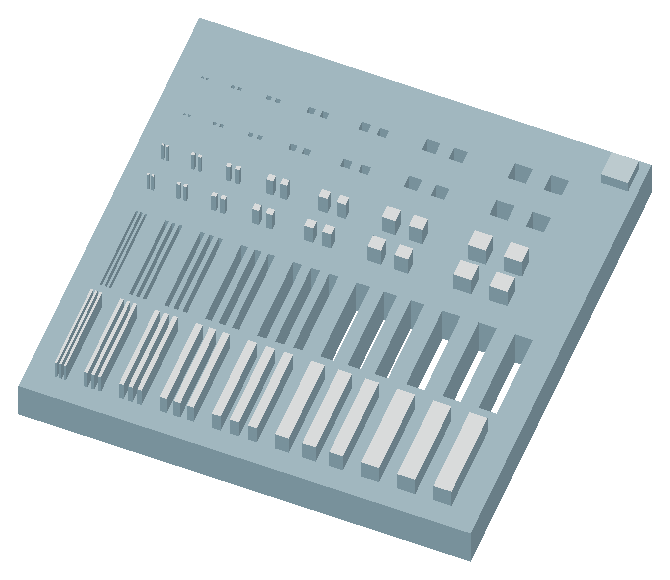
\includegraphics[width=\columnwidth]{figures/xy_resolution_3d_perspective.png}
\caption{Perspective view of the original STL model showing the bars, pillars and openings used to study the XY resolution.}
\label{fig:stl}
\end{figure}

\subsection{Measurement of the working curve}
Following the procedure described in the MNFT-3 guide \cite{vilnius2020mnft3}, liquid resin was placed on a thin microscope slide using a dropper and exposed for different times from 1 to 30~s. After exposure, uncured resin was removed using a bath of isopropyl alcohol. For each of the twenty measurements, the total thickness of the glass and cured resin was measured using a manual caliper. The curing depth was obtained by subtracting the glass thickness of 0.025~cm:
\begin{equation}
\frac{z_p}{\mu\mathrm{m}}=10^4\left(\frac{d_{\mathrm{total}}}{\mathrm{cm}}-0.025\right).
\label{eq:glass}
\end{equation}
The thickness values were recorded in steps of 50~$\mu$m. The measurement at 1~s gave no detectable cured resin and was excluded from the fit.

\subsection{SEM imaging}
Printed samples were imaged using a Hitachi TM-1000 scanning electron microscope. Image calibration from the paired metadata was used for preliminary feature measurements: 0.36719~$\mu$m/pixel at 500$\times$ and 4.58984~$\mu$m/pixel at 40$\times$. The exact positions of the measured features were not recorded. The nominal dimensions used for comparison are therefore estimates based on the STL model.

\section{Results and Discussion}
\subsection{Measured curing depth versus exposure time}
Figure~\ref{fig:rawcuring} shows all 20 corrected curing-depth measurements as a function of exposure time on a conventional linear time axis. The fitted model is shown as a logarithmic curve over the range where resin cured. Although the measured depth generally increases with exposure time, it decreases at some points, for example between 12 and 14~s and between 28 and 30~s. These variations may be related to the manual reading of the caliper and the limited precision of the thickness measurements. The pressure applied by the caliper may also compress the polymer and lead to an underestimate of its thickness. In addition, uncured resin that was not completely removed during cleaning may increase the measured thickness. These effects were not measured separately.

% FIGURE 1 — conventional, non-linearized plot: directly uses corrected CSV.
% Regenerate the fit with: python analysis/plot_working_curve.py
\begin{figure}[h]
\centering
\begin{tikzpicture}
\begin{axis}[
width=.93\linewidth,height=.60\linewidth,
xlabel={Exposure time $t_p$ (s)},
ylabel={Cured resin depth $z_p$ ($\mu$m)},
xmin=0,xmax=31,ymin=-20,ymax=490,
grid=major,
legend style={font=\footnotesize,at={(0.97,0.06)},anchor=south east},
tick label style={font=\small}
]
\addplot+[only marks,mark=*,mark size=1.65pt]
table[col sep=comma,x=exposure_s,y=resin_height_um]
{data/working_curve_corrected.csv};
\addlegendentry{Experimental data}
\addplot+[no marks,thick,domain=1.746:30,samples=150]
{146.122087*ln(x)-81.424785};
\addlegendentry{Logarithmic fit}
\end{axis}
\end{tikzpicture}
\caption{Corrected polymerized resin height versus exposure time, with the logarithmic Jacobs working-curve fit. The measurement at 1~s has zero observed cured thickness and was not included in the regression.}
\label{fig:rawcuring}
\end{figure}

\subsection{Linearized working curve}
Fitting the 19 values with positive curing depth against $\ln(t_p/1\,\mathrm{s})$ gives
\begin{equation}
\frac{z_p}{\mu\mathrm{m}}=146.12\ln(t_p/1\,\mathrm{s})-81.42.
\label{eq:fit}
\end{equation}
The fit gives $h_a=(146.1\pm 7.3)~\mu$m and $T_c=(1.75\pm 0.17)$~s, with $R^2=0.9592$. The uncertainty in $h_a$ is the standard error of the slope. The uncertainty in $T_c$ was obtained by propagating the fit uncertainties, including the covariance between the slope and intercept. Figure~\ref{fig:linearcuring} shows the fit and Fig.~\ref{fig:residuals} shows the residuals. The root mean square of the residuals is 23.4~$\mu$m. These statistical uncertainties do not include systematic errors from the caliper, sample compression or incomplete removal of uncured resin.

% FIGURE 2 — linearized plot. CSV generated by the Python analysis script.
\begin{figure}[h]
\centering
\begin{tikzpicture}
\begin{axis}[
width=.93\linewidth,height=.60\linewidth,
xlabel={$\ln(t_p/1\,\mathrm{s})$},
ylabel={Cured resin depth $z_p$ ($\mu$m)},
xmin=-.1,xmax=3.55,ymin=-20,ymax=490,
grid=major,
legend style={font=\footnotesize,at={(0.03,0.97)},anchor=north west},
tick label style={font=\small}
]
\addplot+[only marks,mark=*,mark size=1.65pt]
table[col sep=comma,x=ln_t_s,y=z_um]
{data/working_curve_fit.csv};
\addlegendentry{Positive-depth data}
\addplot+[no marks,thick,domain=.557:3.5,samples=150]
{146.122087*x-81.424785};
\addlegendentry{Linear regression}
%\addplot+[only marks,mark=x,mark size=2.8pt] coordinates {(0,0)};
%\addlegendentry{No cure at 1 s}
\end{axis}
\end{tikzpicture}
\caption{Linearized working curve. The slope gives $h_a$, and the horizontal intercept gives $\ln(T_c/1\,\mathrm{s})$. The measurement at 1~s with no cured resin was excluded from the fit and is not shown.}
\label{fig:linearcuring}
\end{figure}

% FIGURE 3 — residuals corresponding to the same fitted observations.
\begin{figure}[h]
\centering
\begin{tikzpicture}
\begin{axis}[
width=.93\linewidth,height=.48\linewidth,
xlabel={$\ln(t_p/1\,\mathrm{s})$},
ylabel={Fit residual ($\mu$m)},
xmin=.5,xmax=3.55,grid=major,
tick label style={font=\small}
]
\addplot+[only marks,mark=*]
table[col sep=comma,x=ln_t_s,y=residual_um]
{data/working_curve_fit.csv};
\addplot+[black,no marks,domain=.5:3.55] {0};
\end{axis}
\end{tikzpicture}
\caption{Residuals $z_p-z_{\mathrm{fit}}$ for the data with positive curing depth.}
\label{fig:residuals}
\end{figure}

As requested by the laboratory assignment \cite{vilnius2020mnft3}, Table~\ref{tab:times} reports the exposure times calculated using Eq.~\eqref{eq:prediction}. These are estimates of the exposure times required for the desired curing depths, not independently verified optimal printing settings. The predicted depth of 25~$\mu$m is below the smallest positive measured thickness of 50~$\mu$m. The working curve characterizes the achievable curing depth, which is relevant to axial resolution \cite{vilnius2020mnft3}, but the actual minimum printable layer thickness was not measured.

\begin{table}[h]
\centering
\caption{Predicted exposure times from the preliminary fit of the curing depth.}
\label{tab:times}
\small
\begin{tabular}{@{}cc@{}}
\toprule
Target cured thickness ($\mu$m) & Exposure time (s)\\
\midrule
25 & 2.07\\
50 & 2.46\\
75 & 2.92\\
100 & 3.46\\
125 & 4.11\\
150 & 4.87\\
\bottomrule
\end{tabular}
\end{table}

\subsection{XY resolution}
Figure~\ref{fig:semxy}(a) shows an overview of the printed square structures at 40$\times$ magnification. Figure~\ref{fig:semxy}(b) shows two small openings at 500$\times$ magnification. The openings, originally square, became approximately circular after printing. Their measured horizontal widths were 73.6 and 79.2~$\mu$m, close to the nominal size of 75~$\mu$m. The openings are distinguishable at this scale, but their original shape is not preserved. The rounding may be related to the finite resolution of the projection optics and the curing threshold near the edges of the openings. The individual contributions of these effects were not determined.

Figure~\ref{fig:semxy}(c) shows four bars and the gaps between them at 40$\times$ magnification. Two of the gaps measured 73.4 and 55.1~$\mu$m, close to nominal sizes of 75 and 50~$\mu$m, respectively. The measurements near 75~$\mu$m agree well with each other. The gap near 50~$\mu$m is also visible, but its measurement is less reliable because of the lower SEM magnification and the small number of pixels across the gap (approximately 12). Table~\ref{tab:sem} summarizes these results.

% Labels are placed on the images, including when a file is still pending.
\newcommand{\sempanel}[2]{%
\IfFileExists{figures/#1}{%
\begin{overpic}[width=.94\columnwidth]{figures/#1}
\put(2,78){\colorbox{white}{\small\bfseries (#2)}}
\end{overpic}%
}{%
\begin{minipage}{.94\columnwidth}
\noindent\textbf{(#2)}\par
\centering\optionalimage{#1}
\end{minipage}%
}}

\begin{figure}[h]
\centering
\sempanel{TM-1000_7182(x40).jpg}{a}\par\vspace{2mm}
\sempanel{SEM_7176_annotated.jpg}{b}\par\vspace{2mm}
\sempanel{SEM_7179_annotated.jpg}{c}
\caption{SEM images of the printed XY test structures. (a) Overview of the square structures at 40$\times$. (b) Detail of two rounded openings at 500$\times$. (c) Bars and gaps at 40$\times$.}
\label{fig:semxy}
\end{figure}

\begin{table}[h]
\centering
\caption{Measured widths and estimated nominal dimensions of the smallest features observed in the SEM images.}
\label{tab:sem}
\footnotesize
\begin{tabular}{@{}lrrr@{}}
\toprule
Feature & Nominal & Measured & Error\\
 & ($\mu$m) & ($\mu$m) & (\%)\\
\midrule
Opening H1 & 75 & 73.6 & $-1.87$\\
Opening H2 & 75 & 79.2 & $+5.60$\\
Gap B2--B3 & 75 & 73.4 & $-2.13$\\
Gap B3--B4 & 50 & 55.1 & $+10.20$\\
\bottomrule
\end{tabular}
\end{table}

Under the experimental conditions, features with estimated nominal dimensions of approximately 75~$\mu$m were consistently distinguishable, although their original geometry was not always preserved. A gap with an estimated nominal width of 50~$\mu$m was also visible, but its measurement is less reliable. Since only one scale was printed and the correspondence with the nominal CAD dimensions is approximate, a general minimum XY resolution cannot be established from these measurements.

Figure~\ref{fig:grooves} shows the printed rectangular grooves at 40$\times$ magnification. The feature identified as the fourth groove, counting from the smallest to the largest in the original STL model, was not properly resolved. Instead of a deep rectangular groove, only an irregular and wavy trace was observed on the printed surface. Although the position of the feature can still be identified, its intended geometry was not reproduced. The depth of the groove was not measured. This example shows a case in which the intended geometry was not resolved, even though a trace remained visible.

\begin{figure}[h]
\centering
\optionalimage{TM-1000_7180(x40).jpg}
\caption{SEM image of the rectangular groove structures at 40$\times$ magnification, showing an irregular trace where the intended groove geometry was not resolved.}
\label{fig:grooves}
\end{figure}

\subsection{Additional printed objects}
Two additional objects were printed to observe how the printer reproduces more complex 3D geometries. The first was a small model of Bowser, a character from the Super Mario games. The print was incomplete (Fig.~\ref{fig:printedobjects}(a)). This may be related to the complex geometry of the model and the limited spatial resolution or layer settings of the printer. However, the exact cause of the incomplete print could not be determined.

The second object was a model of the Hubble Space Telescope. Unlike the Bowser model, the telescope was successfully printed (Fig.~\ref{fig:printedobjects}(b)). These two examples show that the quality of the printed object depends on its geometry as well as the printing conditions.

\begin{figure}[h]
\centering
\sempanel{bowser.jpeg}{a}\par\vspace{2mm}
\sempanel{hubble_telescope.jpeg}{b}
\caption{Additional printed objects. (a) Incomplete Bowser model. (b) Successfully printed model of the Hubble Space Telescope.}
\label{fig:printedobjects}
\end{figure}

\section{Conclusions}
The curing depth generally increased with exposure time and was well described by the Jacobs model. The fit gave an effective penetration depth of $(146.1\pm7.3)$~$\mu$m and a critical exposure time of $(1.75\pm0.17)$~s, with statistical uncertainties from the fit. Exposure times were estimated for curing depths from 25 to 150~$\mu$m, but the actual minimum printable layer thickness was not determined. Features with estimated nominal dimensions of approximately 75~$\mu$m were consistently distinguishable in the SEM images. A gap close to 50~$\mu$m was also observed, with lower confidence. Small square openings became rounded, and a rectangular groove was reproduced only as an irregular trace. The Hubble Space Telescope model was successfully printed, while the Bowser model was incomplete.

\bibliographystyle{unsrt}
\bibliography{references}
\end{document}
